\documentclass{uai2023} % for initial submission
% \documentclass[accepted]{uai2023} % after acceptance, for a revised
                                    % version; also before submission to
                                    % see how the non-anonymous paper
                                    % would look like
%% There is a class option to choose the math font
% \documentclass[mathfont=ptmx]{uai2023} % ptmx math instead of Computer
                                         % Modern (has noticable issues)
% \documentclass[mathfont=newtx]{uai2023} % newtx fonts (improves upon
                                          % ptmx; less tested, no support)
% NOTE: Only keep *one* line above as appropriate, as it will be replaced
%       automatically for papers to be published. Do not make any other
%       change above this note for an accepted version.

%% Choose your variant of English; be consistent
\usepackage[american]{babel}
% \usepackage[british]{babel}

%% Some suggested packages, as needed:
\usepackage{natbib} % has a nice set of citation styles and commands
    \bibliographystyle{plainnat}
    \renewcommand{\bibsection}{\subsubsection*{References}}
\usepackage{mathtools} % amsmath with fixes and additions
% \usepackage{siunitx} % for proper typesetting of numbers and units
\usepackage{booktabs} % commands to create good-looking tables
\usepackage{tikz} % nice language for creating drawings and diagrams

%% Provided macros
% \smaller: Because the class footnote size is essentially LaTeX's \small,
%           redefining \footnotesize, we provide the original \footnotesize
%           using this macro.
%           (Use only sparingly, e.g., in drawings, as it is quite small.)

\title{Fast and Scalable Score-Based Calibration Tests}

% The standard author block has changed for UAI 2023 to provide
% more space for long author lists and allow for complex affiliations
%
% All author information is authomatically removed by the class for the
% anonymous submission version of your paper, so you can already add your
% information below.
%
% Add authors
\author[1]{\href{mailto:<jj@example.edu>?Subject=Your UAI 2023 paper}{Jane~J.~von~O'L\'opez}{}}
\author[1]{Harry~Q.~Bovik}
\author[1,2]{Further~Coauthor}
\author[3]{Further~Coauthor}
\author[1]{Further~Coauthor}
\author[3]{Further~Coauthor}
\author[3,1]{Further~Coauthor}
% Add affiliations after the authors
\affil[1]{%
    Computer Science Dept.\\
    Cranberry University\\
    Pittsburgh, Pennsylvania, USA
}
\affil[2]{%
    Second Affiliation\\
    Address\\
    …
}
\affil[3]{%
    Another Affiliation\\
    Address\\
    …
  }

%% Custom additions
\usepackage{preamble}
  
  \begin{document}
\maketitle

\begin{abstract}
We propose the kernel calibration-conditional Stein discrepancy (KCCSD), a new method to estimate and test calibration of probabilistic models.
The method scales linearly with the number of data points, and its test statistics are differentiable and hence can be used as regularizer to obtain better calibrated models.
Moreover, we propose the measure-transport based kernel, a family of score-based kernels on probability distributions.
We employ it in the formulation of the KCCSD to obtain efficient calibration tests for models for which (only) the score-function of the predictions is readily available, including energy-based models and many unnormalized density models in Bayesian inference.
Unlike prior works, our method does not require potentially expensive sampling for calibration evaluation.
We apply our method to train and test the calibration of simulation-based inference models, where calibration is crucial for accurate and robust scientific discoveries.
\end{abstract}

\section{Introduction}\label{sec:introduction}

Calibration is a statistical property of predictive probabilistic models that ensures that a model's prediction matches the conditional distribution of the predicted variable given the prediction.
A calibrated model expresses the uncertainty about its predictions reliably by being neither over- nor underconfident, and hence can be useful even if its accuracy is suboptimal.
In safety-critical applications such as autonomous driving it is crucial that predictive models involved in automatic decision making are neither too under- nor, often more importantly, overconfident.
Unfortunately, empirical studies revealed that popular machine learning models such as deep neural networks tend to trade off calibration for accuracy~\cite{Guo2017}.
This has lead to an increased interest in the study of calibrated models in recent years.

Calibration has been studied in the metereological and statistical literature for many decades~\citep[e.g.,][]{Murphy1977,DeGroot1983}.
For a long time research on calibration has been focused on different notions of calibration for probabilistic classifiers~\citep[e.g.,][]{Murphy1977,DeGroot1983,Platt2000,Broecker2009,Guo2017,Kull2017,kumar18train,Kull2019,widmann2019calibration,vaicenavicius2019evaluating,zadrozny2001obtaining,Naeini2015} and on calibration of quantiles and confidence intervals for real-valued regression problems \citep[e.g.,][]{song2019distribution,Fasiolo2020,Rueda2006,Ho2005,Taillardat2016}.

In recent years, other communities have praised the importance of properties bearing similarities with calibration.
One instance of this is in simulation-based inference (SBI), in which probabilistic models are trained to estimate the posterior of scientific parameters of interest given some observed data.
These posteriors are continuously-valued and hence many existing notions and evaluations of calibration are not applicable.
Therefore the SBI community instead studied the conservativeness of posterior models.
However, the current methods available for assessing conservativeness are very expensive to run, as discussed by \citet{Hermans2021}.
There is thus a clear need for fast and scalable methods that can be used to assess the calibration of continuously-valued predictive models.

In parallel to advances in SBI, multiple works \citep[see, e.g.,][]{song2019distribution,widmann2022calibration} generalized the notion of calibration introduced for probabilistic classifier to continuous-valued predictive models.
In addition, \citet{widmann2022calibration} introduced a kernel-based hypothesis test that outputs, given a predictive model and a validation dataset, whether the model is calibrated.
However, evaluating their test statistic involves computing expectations with respect to the predictions of the model of interest.
These computations can be performed exactly for classification models but in general analytical expressions are available only for specific choices of kernels and models.
At the expense of increasing the variance of the test statistic, one can use unbiased Monte Carlo estimates of the expectations if one can sample from the probabilistic predictions.
Sampling is possible, for instance, if the predictions are modelled by a normalizing flow or variational autoencoder.
However, we argue that in many interesting settings the probabilistic model is intractable and cannot be sampled from in a straightforward way.
For instance, in Bayesian inference, and in particular in SBI models like SNRE~\cite{hermans2020likelihood}, SNLE~\cite{papamakarios2019sequential} and many of their variants, probabilistic predictions are posterior models over a typically multidimensional target variable (e.g., the parameter) which are often unnormalized and require Markov-chain Monte Carlo (MCMC) methods for approximating expectations.
Hence applying the method of \citet{widmann2022calibration} to test for calibration would require running an MCMC algorithm for every data sample used for testing, which is prohibitively expensive.

\paragraph{Contributions} 

In this paper, we introduce the kernel calibration-conditional Stein discrepancy (KCCSD), a new score-based test for
calibration which addresses computational limitations of existing methods.
\begin{itemize}
    \item We first identify that calibration can be understood as a conditional goodness-of-fit problem. This allows us
        to depart from the formulation of~\citet{widmann2022calibration} and
        instead leverage statistical tools from the conditional goodness of fit
        literature investigated by~\citet{jitkrittum2020testing} to formulate a
        new test for calibration based on the KCCSD, which comes with an incomplete
        U-statistic variant that scales linearly with the number of samples.
    \item Second, we focus on the design of kernels to compare unnormalized
        probability distributions, objects which appear in the formulation of our test.
        Such kernels were studied in many works including
        \cite{DBLP:conf/icml/MeunierPC22}, but all require access to empirical
        estimates of the expectations which we assume are expensive to obtain in our setting.
        We propose the measure-transport based kernel, a family of kernels between probability distributions which can be computed using the score-function of the (unnormalized) densities only, without having access to empirical probabilities.
        By considering appropriate special cases, 
        we show this family recovers more traditional kernels as limiting regimes.
    \item Combining our calibration test with our new kernel, we obtain a fast
        scalable calibration test that can be used for a wide class of
        probabilistic models. This test can be used to assess the calibration
        of a model after it was trained, but also as a differentiable
        regularizer to train a calibrated model. We demonstrate the properties
        of our test on synthetic examples, and apply it to problems in
        simulation-based inference, which has become an important consumer of
        calibration methods in recent years~\citep{Hermans2021,delaunoy2022towards}.
\end{itemize}


\section{Background}\label{sec:background}

\paragraph{Notation}
We consider probabilistic systems characterized by a joint distribution $\mathbb{P}(X, Y)$ of random variables $(X, Y)$ taking values in $\mathcal{X} \times \mathcal{Y}$,
and study \emph{probabilistic models} $P_{|\cdot} \colon \mathcal{X} \to \mathcal{P}(\mathcal{Y})$ to approximate the unknown conditional probability of $Y$ given $X = x$: $P_{|x}(\cdot) \simeq \mathbb{P}(Y \in \cdot \,|\, X = x)$.
Target variable $Y$ is typically a parameter of a probabilistic system of interest---like synapses in biological neural networks---while input variable $X$ is observed data---like neuron voltage traces measured using electrophysiology.

\subsection{Calibration of Predictive Models}\label{subsec:calibration}

\paragraph{Calibration: General Definition}

A probabilistic model $P_{|\cdot}$ is called calibrated or reliable~\citep{brocker2008some,zadrozny2001obtaining,widmann2022calibration} if it satisfies
\begin{equation}\label{eq:calibration}
P_{|X} = \mathbb{P}\left(Y \in \cdot \mid P_{|X} \right) \qquad \mathbb{P}(X)\text{-a.s.}.
\end{equation}
Note that this definition applies to general predictive probabilistic models, also beyond classification, and only assumes that the conditional distributions on the left-hand side exist.

\paragraph{Hypothesis Testing: Kernel Calibration Error} 

There are multiple ways to study the calibration of predictive models.
In this section, we introduce the approach of~\citet{widmann2019calibration} and its later generalization~\citep{widmann2022calibration}, on top of which CCKSD is built and on which we focus.
These works introduce kernel-based tests to assess whether a predictive model is calibrated.
These tests turn the equality between conditional-distribution present in \cref{eq:calibration} into a more classical equality between joint distributions.
The transformation is achieved by noting that
\begin{multline}\label{eq:calibration2}
P_{|X} = \mathbb{P}\left(Y \in \cdot \mid P_{|X} \right) \quad \mathbb{P}(X)\text{-a.s.} \\
\iff (P_{|X}, Y) \stackrel{d}{=} (P_{|X}, Z)
\end{multline}
where $Z$ is an ``auxiliary'' variable such that $Z \,|\, P_{|X} \sim P_{|X}(\cdot)$.
This identity between probability distribution was used by \citet{widmann2022calibration} to construct an MMD-type calibration test based on the statistic
\begin{equation}\label{eq:SKCE}
\sup_{h \in \mathcal  B(0_\mathcal{H}, 1)} \E_{(x, y, z) \sim \mathbb{P}(X, Y, Z)} \big[h(P_{|x}, y) - h(P_{|x}, z) \big],
\end{equation}
called the (squared) kernel calibration error~(SKCE).
Here, $\mathcal{B}(0_\mathcal{H}, 1)$ is the unit ball of a reproducing kernel Hilbert space~(RKHS) $\mathcal H$ of functions with positive definite kernel $k_{\mathcal{H}} \colon (P_ {|\mathcal{X}} \times \mathcal{Y})^2  \to \mathbb{R}$.
As noted by \citet{widmann2022calibration}, this formulation generalizes the notion of (squared) kernel classification calibration error~(SKCCE) defined for the special case of discrete output spaces $\mathcal{Y} = \left \{ 1, \dots, d \right \}$  only~\citep{widmann2019calibration}.
\citet{widmann2022calibration} then constructed a test that estimates the SKCE based on $n$ pairs of samples ${\{(P_{|x^i}, y^i)\}}_{i=1}^n \stackrel{\text{i.i.d.}}{\sim} \mathbb{P}(P_{|X}, Y)$:
\begin{equation} \label{eq:SCKE-u-statistics-estimator}
\begin{split}
    &\frac{1}{n(n-1)} \sum\limits_{i \neq j} \Big \{ k((P_{|x^i}, y^i), (P_{|x^j}, y^j)) \\
    & \qquad - \mathbb{E}_{z^i \sim P_{|x^i}} k((P_{|x^i}, z^i), (P_{|x^j}, y^j)) ) \\
    & \qquad - \mathbb{E}_{z^j \sim P_{|x^j}} k((P_{|x^i}, y^i), (P_{|x^j}, z^j))) \\
    & \qquad + \mathbb{E}_{z^i \sim P_{|x^i}} \mathbb{E}_{z^j \sim P_{|x^j}} k((P_{|x^i}, z^i), (P_{|x^j}, z^j)) \Big\}.
\end{split}
\end{equation}

As discussed above and by \citet{widmann2022calibration}, \cref{eq:SCKE-u-statistics-estimator} alludes at two important sources of possible intractability:

\paragraph{First Problem}
The last three terms in the sum are expectations under predictions of the probabilistic model of interest.
However, closed-form expressions for these expectations are only available in restricted cases, such as for classification and for Gaussian models coupled with Gaussian kernels.
When these expectations are not available, they must be approximated numerically.
If the distributions $P_{|X}$ are given in the form of unnormalized models, this approximation requires running expensive approximation methods that often take the form of an MCMC algorithm and must be performed for every sample of $P_{|X}$ used to estimate the test statistic.

\paragraph{Second Problem}
The second source is the choice and evaluation of the kernel function $k$.
We restrict our attention to the conventional form of tensor-product type kernels $k((p, y), (p', y')) = k_{P}(p, p') k_{Y}(y, y')$ chosen in this setting.
While typically many tractable choices for the kernel $k_{Y}$ exist (taking as input discrete or Euclidean values), the choices for $k_{P}$, defined for two probability distribution $p$ and $p'$, are more limited and require expensive approximations methods when working with unnormalized models.

A popular approach to design kernels on distributions~\citep{DBLP:journals/jmlr/SzaboSPG16, DBLP:conf/aistats/0001GPS15} is to first embed the probability distributions in an Hilbert space $\mathcal{H}$ using a map $\phi$, and then compose it with a kernel $k_{\mathcal{H}}$ on $\mathcal{H}$:
\begin{equation*}
k_{P}(p, p') = k_{\mathcal{H}}(\phi(p), \phi(p')).
\end{equation*}
Any valid  kernel on $ \mathcal{H}$, like the linear kernel $k_{\mathcal{H}}(z, z') = \left \langle z, z' \right \rangle_{\mathcal{H}}$, the Gaussian kernel $k_{\mathcal{H}}(z, z') = e^{-\left \|z - z'\right \|^2_{\mathcal{H}}}$, or the multiquadric kernel $k_{\mathcal{H}}(z, z') = (1 + \left \|z - z'\right\|^2_{\mathcal{H}})^{-1}$ can be used.
In practice, the map $\phi$ can be set to be the \emph{mean embedding} map to an RKHS $\mathcal{H}$, e.g., $\phi(\mu) = \int k_{\mathcal{H}}(z, \cdot) \,\mu(\mathrm{d}z)$.
Kernels $k_{\mathcal{H}}$ that are functions of $\left\| \phi(\mu) - \phi(\nu) \right \|^2_{\mathcal{H}} := \operatorname{MMD}^2(\mu, \nu)$, are often referred to as MMD-type kernels~\cite{DBLP:conf/icml/MeunierPC22}.
Other distances, like the Wasserstein distance in 1 dimension or the sliced Wasserstein distance~\citep{DBLP:journals/jmiv/BonneelRPP15} in multiple dimensions, also take this form for some choice of $\phi$ and $\mathcal{H}$, and can thus be used to construct kernels on distributions~\cite{DBLP:conf/icml/MeunierPC22}.
In general, however, estimating $k_{P}(p, p')$ becomes intractable apart from special cases such as when $p$ and $p'$ are Gaussian distributions.
\textbf{While there exist finite-samples estimators for such kernels, a fast calibration estimation method based on \cref{eq:SKCE} would require an estimator that does not require samples from $p$ and $p'$}.


% Finally, as noted by
% \cite{widmann2022calibration}, these kernels can also be used in the
% case where the distributions of interest can be injectively described by a
% vector $ \phi(p) \in \mathbb{R}^d $, although the last setting rarely happens in practical cases.


% \begin{equation} \label{eq:classification-SKCE}
% \begin{aligned}
% \text{SKCCE}((Y, g(X)), (Z, g(X))) &= \sup_{ h \in \mathcal  H_d } \mathbb{E}_{  }\left [ (r(g(X)) - g(X))^{\top}h(g(X)) \right ] 
% \end{aligned}
% \end{equation}
% where $ r $ is the \emph{Canonical Calibration Function} as defined in \cite[Equation 4]{vaicenavicius2019evaluating}:
%  \begin{equation*}
% \begin{aligned}
%     r: \mathcal  P(\mathcal  Y) &\longrightarrow  \mathcal  P(\mathcal  Y) \\
%       g(X) &\longmapsto r(g(X)) = \mathbb{E}_{  }\left [ Y | g(X) \right ] 
% \end{aligned}
% \end{equation*}
% and $ \mathcal  H_d $ is a \emph{vector valued} RKHS with kernel $ K $:
% \begin{equation*}
% \begin{aligned}
%     K:P(\mathcal  X) \times \mathcal  P(\mathcal  X)    &\longrightarrow \mathbb{R}^{d \times d} \\
%     (p, p')&\longmapsto K = (k((p, i), (p', j)))_{ij}.
% \end{aligned}
% \end{equation*}


\subsection{Calibration beyond Classification: Application in Bayesian Inference}

\paragraph{Bayesian Inference and SBI}
One main motivation for studying calibration of generic probabilistic models is Bayesian inference,
which seeks to compute the (approximate) posterior distribution of a parameter $y$ of interest given some observed variable $x$.
These posterior distributions are special instances of probabilistic models $P_{|x}$, depending on the observed data $x$, and thus calibration tests can be used to assess the calibration of these Bayesian models.
In the case of SBI, a family of Bayesian inference approaches particularly popular in
scientific domains such as neuroscience or physics, it is particularly
important that the posterior estimate exhibits reliability properties as
non-reliable models can cause incorrect scientific conclusions. As shown 
by~\citet{Hermans2021} such reliability properties are not always verified by the
approximate posteriors returned by SBI methods. Unfortunately, the reliability
evaluation process is complicated by the fact current reliability
estimation methods are very costly to run~\cite{Hermans2021}. Thus it is
crucial to provide the Bayesian inference community with practical and fast
reliability estimation methods.

\paragraph{Reliability in Bayesian Inference versus Calibration}
It is important to note that reliability metrics traditionally
used in Bayesian inference such as posterior coverage~\cite{Hermans2021}
differ from the notion of calibration in \cref{eq:calibration}.
However, in \cref{sec:fast-calibration-tests} we show that a probabilistic model that is calibrated according to \cref{eq:calibration} is also reliable in the sense of \citet{Hermans2021}, grounding the use of our tests in Bayesian inference.

\subsection{Kernel Conditional Goodness-of-Fit Test}

\emph{Conditional goodness-of-fit} (or CGOF) testing tests whether 
\begin{equation}\label{eq:cgof-hypothesis}
H_0\colon P_{|X} = \mathbb{P}(Y \in \cdot \,|\, X) \qquad \mathbb{P}(X)\text{-a.s.}
\end{equation}
given a model $P_{|x}$ for the conditional distribution $\mathbb{P}(Y \in \cdot \,|\, X=x)$ and samples ${\{(x^{i}, y^{i})\}}_{i=1}^n \stackrel{\text{i.i.d}}{\sim} \mathbb{P}(X, Y)$.
This problem was studied by \citet{jitkrittum2020testing} for the case $\mathcal{X} \times \mathcal{Y} \subset \mathbb{R}^{d_x} \times \mathbb{R}^{d_y}$ and models $P_{|x}$ with a differentiable, strictly positive density $f_{P_{|x}}$.
They proposed a kernel CGOF test for \cref{eq:cgof-hypothesis} based on the (squared) kernel conditional Stein discrepancy~(KCSD)
\begin{equation}\label{eq:cgof-metric}
    D_{P_{|\cdot}}(\mathbb{P}) := \left \| \mathbb{E}_{(x,y) \sim \mathbb{P}(X, Y)}\left [ K_{x} \xi_{P_{|x}}(y, \cdot) \right ]  \right \|^2_{\mathcal  F_{K}}
\end{equation}
where
\begin{itemize}
    \item $\mathcal  F_{l} $  is an RKHS on $ \mathcal  Y $ with kernel $l \colon \mathcal{Y} \times \mathcal{Y} \to \mathbb{R}$ and $ \mathcal  F^{d_{y}}_l = \otimes_{d_y} \mathcal  F_{l}$,
    \item $\xi_{P_{|x}} $ is the ``kernelized score''
	\begin{equation*}
	    \xi_{P_{|x}}(y, \cdot) = l(y, \cdot)\nabla_{ y } \log f_{P_{|x}}(y) + \nabla_{ y }  l(y, \cdot) \in \mathcal F_{l}^{d_y},
	\end{equation*}
    \item $ \mathcal  F_{K} $ is an $F^{d_y}_{l}$-vector-valued RKHS with kernel
	$K\colon \mathcal{X} \times \mathcal{X}  \to \mathcal{L}(\mathcal{F}^{d_y}_{l}, \mathcal{F}^{d_{y}}_{l})$, and
    \item $K_{x}$ is its associated linear operator on $ \mathcal  Y $:
    \begin{equation*}
    \begin{aligned}
	K_{x} \colon  \mathcal  Y&\longrightarrow \mathcal  L(\mathcal{X}, \mathcal{Y}), \\
	 y &\longmapsto K_{x} y = K(x, \cdot)y.
    \end{aligned}
    \end{equation*}
\end{itemize}

Under certain assumptions~\citep[Theorem~1]{jitkrittum2020testing}, such as kernels $K$ and $l$ being $C_0$-universal,
the null hypothesis in \cref{eq:cgof-hypothesis} is true if and only if $D_{P_{|\cdot}}(\mathbb{P}) = 0$.
An example of an $\mathcal
F^{d_y}_l$-reproducing $C_0$-universal kernel $K$ is
\begin{equation}\label{eq:kernel_identity}
K(x, x') = k(x, x')I_{\mathcal{F}_l^{d_y}}
\end{equation}
where $I_{\mathcal{F}_l^{d_y}} \in \mathcal  L(\mathcal  F^{d_y}_l, \mathcal  F^{d_y}_{l})$ is the identity operator and $k$ is a real-valued $C_0$-universal kernel~\citep{carmeli2010vector}.
\citet{jitkrittum2020testing} showed that the CGOF statistic $D_{P_{|\cdot}}(\mathbb{P})$
admits an unbiased consistent estimator and used it to construct hypothesis tests of \cref{eq:cgof-hypothesis} with operator-valued kernels of the form in \cref{eq:kernel_identity}.
%$\widehat{D_{\widehat{P}}}$ given by
%\begin{equation*}
%\widehat{D_{\widehat{P}}} = \frac{2}{n(n-1)} \sum\limits_{1 \leq i < j \leq n} k(x^i, x^j) h_{\widehat{p}}((x^i, y^i), (x^j, y^j))
%\end{equation*}
%where    
%\begin{equation}\label{eq:gof-test-statistics}
%\begin{split}
%    &h_{\widehat{p}}((x, y), (x', y')) := l(y, y') s_{\widehat{p}}(x, y)^{\top} s_{\widehat{p}}(x', y') \\
%    &\qquad+ \sum\limits_{ i=1 }^{ d_y } \frac{ \partial^2 }{ \partial y_i \partial y_i' } l(y, y')
%    + s_{\widehat{p}}(x, y)^{\top} \nabla_{ y' } l(y, y')\\
%    &\qquad + s_{\widehat{p}}(x', y')^{\top} \nabla_{ y } l(y, y'),
%\end{split}
%\end{equation}
%and $s_{\widehat{p}}(x, y) := \nabla_{y} \log \widehat{p}(x)(y)$.
%\citet{jitkrittum2020testing} use $\widehat{D_{\widehat{p}}}$ to construct hypothesis tests that check \cref{eq:cgof-hypothesis}.

\section{Kernel Calibration-Conditional Stein Discrepancy}\label{sec:calibration-as-cgof}

Calibration testing in the sense of \cref{eq:calibration} is an instance of \emph{conditional goodness-of-fit} testing of \cref{eq:cgof-hypothesis} with input $P_{|X}$, target $Y$, and models $P_{|x} \mapsto P_{|x}$.
%Interestingly, under the null hypothesis, the conditional probability $p(y \,|\, g(x)) $ admits a tractable form since under $ H_0 $, $ p(y|g(x)) = \big[\frac{\mathrm{d}}{\mathrm{d}\nu} g(x)\big](y) \eqqcolon \gamma(x)(y)$ where $\gamma(x)$ is the density of $g(x)$ with respect to a base measure $\nu$ (independent of $x$).
Assuming that $\mathcal{Y} \subset \mathbb{R}^{d_y}$ and that distributions $P_{|x}$ have a differentiable, strictly positive density $f_{P_{|x}}$,
thus the (squared) kernel conditional Stein discrepancy in \cref{eq:cgof-metric} becomes
\begin{equation}\label{eq:calibration-cgof-metric}
    C_{P_{|\cdot}}(\mathbb{P}) := \left \| \mathbb{E}_{(x,y) \sim \mathbb{P}(X, Y)}\left [ K_{P_{|x}} \xi_{P_{|x}}(y, \cdot) \right ]  \right \|^{2}_{\mathcal  F_{K}},
\end{equation}
where now $K$ is a kernel on $P_{|\mathcal{X}}$.
To emphasize the calibration setting, we call $C_{P_{|\cdot}}$ the kernel calibration-conditional Stein discrepancy~(KCCSD).
Similar to the KCSD, given samples ${\{P_{|x^i}, y^i\}}_{i=1}^n \stackrel{\text{i.i.d.}}{\sim} \mathbb{P}(P_{|X}, Y)$ and assuming a kernel $K$ of the form in \cref{eq:kernel_identity}, statistic $C_{P_{|\cdot}}(\mathbb{P})$ has an unbiased consistent estimator
\begin{equation*}\label{eq:calibration-gof-estimator}
    \widehat{C_{P_{|\cdot}}} = \frac{2}{n(n - 1)} \sum_{1 \leq i < j \leq n} H((P_{|x^i}, y^i), (P_{|x^j}, y^j))
\end{equation*}
where
\begin{equation}\label{eq:calibration-cgof-test-statistic}
    H((p, y), (p', y')) := k(p, p') h((p, y), (p', y'))
\end{equation}
with
\begin{equation}\label{eq:calibration-cgof-test-statistic-h}
\begin{split}
    &h((p, y), (p', y')) := l(y, y') s_p(y)^{\top} s_{p'}(y') \\
    &\qquad+ \sum\limits_{i=1}^{d_y} \frac{\partial^2}{ \partial y_i \partial y_i'} l(y, y')
    + s_p(y)^{\top} \nabla_{y'} l(y, y') \\
    &\qquad+ s_{p'}(y')^{\top} \nabla_{y} l(y, y'),
\end{split}
\end{equation}
where $s_{p}(y) := \nabla_y \log f_{p}(y)$ (resp.\ $s_{p'}(y)$) is the \emph{score} of $p$ (resp.\ $p'$).
In \note{Section~A} in the supplement we discuss how the formula of $\widehat{C}_{P_{|\cdot}}$ generalizes to operator-valued kernels that are not of the form in \cref{eq:kernel_identity}.

The above framing of the calibration problem conveniently avoids the first source of possible intractability present in the SKCE.
For instance, for Gaussian models the test statistic can be evaluated exactly for arbitrary kernels $l$ on $\mathcal{Y}$ whereas a closed-form expression of the SKCE is known only in the special case where $l$ is a Gaussian kernel.

\Cref{prop:kccsd-relation-skce} shows that the KCCSD can be viewed as a special case of the SKCE.
More generally, as shown in \note{Section~B}, the KCSD is a special form of the MMD.

\begin{proposition}[Special case of \note{Lemma~B.1}]\label{prop:kccsd-relation-skce}
Under weak assumptions (see~\note{Lemma~B.1}),
the KCCSD with respect to kernels $l \colon \mathcal{Y} \times \mathcal{Y} \to \mathbb{R}$ and $k \colon P_{|\mathcal{X}} \times P_{|\mathcal{X}} \to \mathbb{R}$ is equivalent to the SKCE with kernel $H \colon (P_{|\mathcal{X}} \times \mathcal{Y}) \times (P_{|\mathcal{X}} \times \mathcal{Y}) \to \mathbb{R}$ defined in \cref{eq:calibration-cgof-test-statistic}.
\end{proposition}

\paragraph{Linear Time Variants}
The minimum-variance estimator of this U-statistic requires $n(n-1)$ evaluations and thus scales quadratically with the sample size.
Therefore in our tests we employ linear-time tests variants, based on incomplete
U-statistics estimation~\cite{schrab2022efficient} or on B-tests~\cite{zaremba2013b}.
Indeed, sample sizes in typical Bayesian application are such that operations of with a complexity scaling quadratically with the numbers of samples are intractable on commodity hardware.
These linearization methods are conceptually similar to their quadratic counterparts, and do not require solving an additional optimization problem, as the test points methods of \citet{jitkrittum2020testing,jitkrittum2017linear}.

\note{I think we need to do the theory if we actually use incomplete
U-statistics linearization?}

The full testing procedure is outlined in \cref{alg:ccgof-tractable}.
The computations can be performed with kernels $K$ of the form in \cref{eq:kernel_identity} or more general operator-valued kernels, but crucially the method requires that $K$ is tractable.
Thus for general models of probability distributions, such as energy-based models and other unnormalized density models, it remains to address the second source of intractability, namely to construct a kernel $K$ that can be evaluated efficiently.

\begin{algorithm}
    \DontPrintSemicolon
    \caption{CGOF Calibration Test (Tractable Kernel)}\label{alg:ccgof-tractable}
	\KwData{Pairs ${\{(P_{|x^i}, y^i)\}}_{i=1}^n \stackrel{\text{i.i.d.}}{\sim} \mathbb{P}(P_{|X}, Y)$}
	\KwResult{Whether to reject $H_0 \colon \text{``model is calibrated''}$}
    \Parameters{Number of data samples $n$, kernel $l \colon \mathcal{Y}^2 \to \mathbb{R}$, kernel $k \colon (P_{|\mathcal{X}})^2 \to \mathbb{R}$, set of indices pairs $R \subset \left\{ 1, \ldots, n \right\}^{2}$, significance level $\alpha$}
    \BlankLine
    \tcc{Estimate KCCSD using \cref{eq:calibration-cgof-test-statistic-h} or \note{(A.1)}}
    $\widehat{C} \leftarrow \frac{1}{\lvert R \rvert } \sum\limits_{ (i, j) \in R } H((P_{|x^i}, y^i),(P_{|x^j}, y^j))$\;
    \tcc{Use e.g.\ bootstrap~\citep{schrab2022efficient}}
    $\widehat{C}_{\alpha} \leftarrow$ approximate $(1- \alpha)$-quantile of $\widehat{C}$\;
    \eIf{$ \widehat{C} < \widehat{C}_{\alpha}$}{%
        \Return{Fail to reject $H_0$}%
    }{%
        \Return{Reject $H_0$}%
    }
\end{algorithm}


\section{Tractable Kernels for General Unnormalized Densities}\label{subsec:expgfd-kernel}


In this section, we introduce two kernels between (density-based) probability
distributions that admit unbiased estimates that neither require samples from
the said distributions nor require access their normalizing constant.
Crucially, the properties of these new kernels allow to extend the scope of calibration
tests to a larger setting, including Bayesian inference.

\paragraph{General Recipe} 
As in prior work on kernels for distributions~\citep{DBLP:conf/icml/MeunierPC22,DBLP:journals/jmlr/SzaboSPG16},
our proposed kernels take the form of exponentiated Hilbertian metrics
\begin{equation*}
k(p, q) = e^{- \left \| \phi(p) - \phi(q) \right \|^2_{H} / (2\sigma^2)}
\end{equation*}
where $ H $ is some Hilbert space, $ \phi \colon p \mapsto \phi(p) \in H $ is a
feature map, and $ \sigma $ is a bandwidth parameter.
Our contributions in this section consist in pairs of carefully
designed $ \phi $ and $ H $ that will allow approximating $ k $ easily.


%\subsubsection{The Gene}
%Our starting point
%\subsection{The Generalized Fisher Divergence}
\paragraph{Tractable Hilbertian Distances between unnormalized densities}

Our starting point is the
\emph{Fisher Divergence}~\citep{lyu2012interpretation,sriperumbudur2017density,hyvarinen2005estimation}, also known as the \emph{Relative Fisher Information}~\citep{otto2000generalization}, between two probability densities $ p $ and $ q $, which is given by
\begin{equation*}\label{eq:fd}
    \operatorname{FD}(p, q) := \int_{\mathcal  X} \left \| s_p(x) - s_q(x)  \right \|^2 p(x) \,\mathrm{d}x.
\end{equation*}
The Fisher Divergence is a convenient tool to compare unnormalized densities of the form
\begin{equation*}
p(x):= \frac{ \overbrace{f(x)}^{\text{tractable}} }{ \underbrace{Z_f}_{\text{intractable}} } \quad \text{where} \quad Z_f:= \int_{\mathcal  X} f(x) \,\mathrm{d}x
\end{equation*}
as the score of $ p $ can be evaluated without knowing $ Z_f $:
\begin{equation*}
    s_p(x) = \nabla_{x} (\log f(x)/{Z_f}) = \nabla_{x} \log f(x).
\end{equation*}
This property confers the Fisher Divergence with a tractable unbiased
estimator given $ n $ i.i.d.\ samples $ \{X^{i}
\}_{i=1}^{n} $ from $ p $, which takes the form:
\begin{equation*}
    \widehat{\operatorname{FD}(p, q) } = \frac{1}{n} \sum_{i=1}^{n} \|  s_p(X^{i}) - s_q(X^{i})  \|^2.
\end{equation*}
While the assumption
ensuring access to samples from $ p $ is realistic in the unsupervised learning
literature~\citep{hyvarinen2005estimation}, or when dealing with special
instances of unnormalized densities such as truncated densities $ f(x) = p(x)\textbf{1}_{x \in
\mathcal  C}  $, it does not hold in the context of studying the calibration of
unnormalized models, where the samples $ y^{i} $ are drawn from the unknown
$ p^{\star}(y|x^{i}) $, which may or may not equal the model $ p(y|x^{i}) $.
We overcome this issue by constructing a generalized version of the Fisher Divergence:
\begin{definition}[Generalized Fisher Divergence]
    Let $ p $,  $ q $ be two probability densities on $ \mathcal  X $, and
    $ \nu $ a probability measure on $ \mathcal  X $. The \emph{Generalized
    Fisher Divergence} between $ p $ and $ q $ is defined as
\begin{equation*} \label{eq:gfd}
\operatorname{GFD}_{\nu}(p, q) := \int_{\mathcal  X} \left \| s_p(x) - s_q(x)  \right \|^2 \,\nu(\mathrm{d}x),
\end{equation*}
if $ \mathbb{E}_{ \nu }\left \| s_p  \right \|^2, \mathbb{E}_{ \nu }\left \|
s_q  \right \|^2 < +\infty $, and $ +\infty $ otherwise.
\end{definition}
The Generalized Fisher Divergence differs from the Fisher Divergence in that
the integration is performed with respect to some given base measure $ \nu $
instead of $ p $. If the support of $ \nu $ covers the support of $ p $ and $ q
$,  then we have that $ \operatorname{GFD}_{\nu}(p, q) = 0 $ iff.\ $ p = q $.
Moreover, if $ \nu $ can be sampled from in a tractable manner, then $
\operatorname{GFD}_{\nu}(p, q)$ admits a tractable estimator given samples $ \{ Z^{i}
\}_{i=1}^{n}  $ from $ \nu $ of the form
\begin{equation*}
\widehat{ \operatorname{GFD}}_{\nu}(p, q) = \frac{1}{n} \sum_{i=1}^{n} \| s_p(Z^{i}) - s_q(Z^{i})  \|^2.
\end{equation*}
In practice, the tractability assumption as well as the support assumption for
any $ p $, $ q $ are verified by setting $ \nu $ to be a standard Gaussian
distribution.
%We discuss in more detail in \cref{subsec:experiments-synthetic} the tuning of the base measure $ \nu $.

%\subsection{Calibration tests based on the Generalized Fisher Divergence}

\paragraph{The Exponentiated-GFD Kernel}

Importantly, the (square root of
the) Generalized Fisher Divergence is a Hilbertian metric on the space
of probability densities.
Indeed, for $ p $, $ q $ such that $ \mathbb{E}_{ \nu } \left \| s_p  \right
\|^2, \mathbb{E}_{ \nu } \left \| s_q  \right \|^2 < +\infty $, we have that
\begin{equation*}
\operatorname{GFD}_{\nu}(p, q) = \left \| \phi(p) - \phi(q) \right \|_{\mathcal  L_2(\nu)}^{2}
\end{equation*}
where $ \phi \colon p  \mapsto s_p(\cdot) \in \mathcal L_2(\nu)  $.
The latter fact allows to construct a kernel $ K_{\nu} $ on the space of
probability densities based on the Generalized Fisher Divergence as follows:
\begin{definition}[Exponentiated GFD Kernel]\label{def:expgfdkernel}
    Let $ p $,  $ q $ be two probability densities on $ \mathcal  X $, and
    $ \nu $ a probability measure on $ \mathcal  X $. The \emph{exponentiated
    GFD kernel} between $ p $ and $ q $ is defined as
\begin{equation*}
    K_{\nu}(p, q) := e^{ - \operatorname{GFD}_{\nu}(p, q)/ (2\sigma^2)}
\end{equation*}
\end{definition}
Since the $\operatorname{GFD} $ is a Hilbertian metric, $ K_{\nu} $ is positive
definite~\citep{DBLP:conf/icml/MeunierPC22}, and can be estimated given samples
of $ \nu $ by replacing $ \operatorname{GFD}_{\nu} $ with its empirical counterpart. We
summarize the computation method for $ K_{\nu} $ in \cref{alg:expgfdkernel}.

\begin{algorithm}
    \DontPrintSemicolon
    \caption{Exponentiated GFD Kernel}\label{alg:expgfdkernel}
    \KwData{Probability densities $p, q$ on $\mathcal{X}$}
	\KwResult{Approx. $\widehat{K_{\nu}(p, q)}$ of $K_{\nu}(p, q)$ in \cref{def:expgfdkernel}}
	\Parameters{Base measure $\nu$, num. of base samples $m$}
    \BlankLine
	\For{$i \leftarrow 1$ \KwTo $m$}{
        Draw $Z^i \sim \nu$\;
    }
    \Return{$\exp{\left(- \frac{1}{2m \sigma^2} \sum_{i=1}^{m} \|  s_p(Z^{i}) - s_q(Z^{i})\|^2\right)}$}\;
\end{algorithm}

Note the difference in the estimation error of such kernels compared to
traditional MMD-type kernels of the form
\begin{equation*}
K_{\operatorname{MMD}}(p, q) = e^{ - \operatorname{MMD}^2(p, q)/ (2\sigma^2)}.
\end{equation*}
In the GFD case, the error arises from discretizing $\nu$ whereas in the second
case the error is caused by approximating $p$ and $q$ by samples, i.e., by setting $\widehat{K_{\operatorname{MMD}}(p, q) } := K_{\operatorname{MMD}}( \widehat{ p }, \widehat{ q }) $.

\paragraph{Kernelizing the Generalized Fisher Divergence}

While the recipe given above suffices to obtain a valid kernel on the space of
probability densities, the approximation error arising from the discretization
of the base measure $\nu$ may scale unfavorably with the dimension of the
underlying space $\mathcal{X}$. To address this issue, it is possible to apply
a kernel-smoothing step to the GFD feature map $ \phi(p) $ by composing it with
an integral operator $ T_{K, \nu} $ associated with a $ \mathcal  X
$-vector-valued kernel $ K $ and its RKHS $ \mathcal  H_{ K} $
\begin{equation*}
T_{K, \nu} \colon f \in \mathcal  L(\mathcal  X, \mathbb{R}^d)  \longmapsto \int_{\mathcal{X}} K_x f(x)  \, \nu(\mathrm{d}x) \in \mathcal  H_{ K}
\end{equation*}
and comparing the difference in feature map using the squared RKHS norm $ \left
\| \cdot \right \|_{\mathcal{H}_K}^{2} $. This choice of feature map yields
another metric, which we call the ``kernelized'' GFD:
\begin{equation*}
\operatorname{KGFD}(p, q) := \left \| T_{K, \nu} s_p - T_{k, \nu} s_q \right \|_{\mathcal  H_{K}}^{2}.
\end{equation*}
It admits the following sample-based estimator:
\begin{equation*}
%    \widehat{\text{KGFD}}(p, q)\hspace{-0.2em} &= \hspace{-0.3em} \frac{1}{m^2}
%    \hspace{-0.4em}\sum_{i,j=1}^{m} \hspace{-0.3em} \left \langle  K(Z^{i},
%    Z^{j}) s_p(Z^{i}), s_q(Z^{j}) \right \rangle_{\mathcal  X} \\
    \frac{1}{m^2}
    \sum_{i,j=1}^{m}\left \langle  K(Z^{i},
    Z^{j}) (s_p - s_q)(Z^{i}), (s_p - s_q)(Z^{j}) \right \rangle_{\mathcal  X}.
\end{equation*}
The kernelized GFD is also a Hilbertian metric. Moreover, for characteristic
kernels $ K $, the integral operator $ T_{K,\nu} $ is a Hilbertian isometry
between $ \mathcal  L_2(\nu)^{\otimes d}$ and $ \mathcal  H_{K} $, making the
exponentiated KGFD kernel positive definite.

\subsection{A diffusion interpretation of the Generalized Fisher Divergence}
In this section, we further analyze the properties of the GFD by establishing a
link with diffusion processes. This link further anchors the GFD to the
array of previously known divergences, while opening the door for possible
refinements and generalizations of the GFD.
\paragraph{A Dissipation Inequality}
Diffusion processes~\citep{rogers2000diffusions} are well-known instances of
stochastic processes $ (X_t)_{t \geq  0} $ that evolve from some
initial distribution $ \mu_0 $ towards a target distribution $ p $ according to
the differential update rule
\begin{equation*}
    \mathrm{d}X_t = s_p(X_t) \,\mathrm{d}t + \mathrm{d}W_t, \quad X_0 \sim \mu_0.
\end{equation*}
For any time $ t \geq  0 $, the probability density of $ X_t $ is the solution $\mu_{\mu_0, p}(\cdot, t)$
of the so-called Fokker-Planck equation
\begin{equation}\label{eq:fp}
    %\mu(x, 0) &= \nu(x),\\
    \frac{\partial \mu(x, t)}{\partial t} = \operatorname{div}(-\mu(x, t) s_p(x)) + \Delta_x \mu(x, t)
\end{equation}
with initial condition $ \mu(\cdot, 0) = \mu_0 $.
\cref{prop:link-kl-gfd} establishes a link between these solutions and the GFD:

\begin{proposition}[Diffusion interpretation of the GFD]\label{prop:link-kl-gfd}
    %Assume that $ p $ and  $ q $ have Lipschitz gradients, and that
    %$ \nu(x) = o(x^{-(1+\alpha)}) $ for some $ \alpha > 0 $.
    Let $\mu_{\nu, p} $ (resp.\ $ \mu_{\nu, q} $)
    be the solution of \cref{eq:fp} with initial
    condition $ \nu $ and target $ p $ (resp.\ $q$). Let $ k $ be a \emph{real-valued},
    twice-differentiable kernel.
    Then, we have that
    \begin{equation*}
        \lim_{t \to 0} \frac{1}{t}\operatorname{MMD}(\mu_{\nu, p}(\cdot, t), \mu_{\nu, q}(\cdot, t)) = \sqrt { \operatorname{KGFD}(p, q) } 
    \end{equation*}
    where the $ \operatorname{MMD} $ is w.r.t.\ the kernel $ k $, and the $\operatorname{KGFD}$ is with respect to the matrix-valued kernel
    $ \nabla_{x} \nabla_{ y } k(x, y) $.
\end{proposition}
\begin{proof}
    %See \cref{app-sec:limit-fisher-divergence}
    See \note{Section~D} of the Appendix.
\end{proof}
\cref{prop:link-kl-gfd} frames the exponentiated KGFD kernel as the $ t  \to 0
$ limit of the kernel obtained by setting
\begin{equation*}
\phi_t \colon p  \longmapsto \nabla_x \log \mu_{\nu, p}(\cdot, t)
\end{equation*}
which is the score of the solution of the Fokker-Planck equation~\cref{eq:fp}
with target $ p $ and initial measure $ \nu $, and setting $ H = \mathcal  H $.
Interestingly, the other limit case $ t  \to \infty $ recovers 
the exponentiated MMD kernel.
Indeed, under mild conditions, the Fokker-Planck solution converges to the
target and thus we have that $ \lim_{  t \to \infty }\phi_t(p) = p  $: the
feature map converges to the identity. Thus, the diffusion framework introduced
above allows to recover both the $ \operatorname{KGFD} $ and the $ \operatorname{MMD} $ as
special cases. However, while the limit $ t  \to 0 $ and $ t  \to \infty $
yield both Hilbertian metrics, it is an open question whether for a given time
$0 < t < \infty$,  $ \phi_t $ is also Hilbertian. A positive answer to this question would
allow to construct positive definite kernels that can possibly overcome the
pitfalls of score-based tools~\citep{wenliang2020blindness, zhang2022towards},
while being computable in finite time.

\section{Fast and scalable calibration tests}\label{sec:fast-calibration-tests}

The framing of the calibration testing problem of \cref{sec:calibration-as-cgof} alongside with the GFD-based kernels of \cref{subsec:expgfd-kernel} allows us to design a fast and scalable alternative to the pioneering tests of \citet{widmann2019calibration}.
The full testing procedure is outlined in \cref{alg:ccgof}.

\begin{algorithm}
    \DontPrintSemicolon
    \caption{CGOF Calibration Test (GFD Kernel)}\label{alg:ccgof}
    \KwData{Pairs ${\{(P_{|x^i}, y^i)\}}_{i=1}^n \stackrel{\text{i.i.d.}}{\sim} \mathbb{P}(P_{|X}, Y)$}
    \KwResult{Whether to reject $H_0 \colon \text{``model is calibrated''}$}
	\Parameters{Base measure $\nu$, number of base samples $m$, number of data samples $n$, kernel $l \colon \mathcal{Y}^2 \to \mathbb{R}$, set of indices pairs $R \subset \lbrack \left \{ 1, \ldots, n \right \} \rbrack^{2}$, significance level $\alpha$}
    \BlankLine
    \For{$i \leftarrow 1$ \KwTo $m$}{%
        Draw $z^i \sim \nu$\;
    }
    \For{$(i, j) \in R$}{%
        \tcc{Use \cref{alg:expgfdkernel} with base samples $\{z^k\}_{k=1}^m$}
        $\kappa^{i,j} \leftarrow \widehat{K_{\nu}(P_{|x^i}, P_{|x^j})}$\;
    }
    Run \cref{alg:ccgof-tractable} with kernel $k(P_{|x^i}, P_{|x^j}) := \kappa^{i,j}$\;
\end{algorithm}

\paragraph{Use as a Regularizer} 
We additionally propose to use this statistic as a calibration regularizer
during the training procedure of a probabilistic model. Because the plug-in
estimator of $ D_p $ using the proposed kernels is cheap to compute and
differentiable, adding this regularizer adds little overhead to the entire
procedure and allows us to train calibrated models instead of simply
diagnosing calibration of existing models.

\section{Related Work}\label{sec:related-work}

The conservativeness of SBI posterior models was first investigated by \citet{Hermans2021}.
The authors introduced the notion of \emph{expected coverage probability}, which can be seen as a consequence of calibration in the sense of \citet{vaicenavicius2019evaluating}, as shown in \cref{sec:fast-calibration-tests}.
\citet{Hermans2021} highlighted the computational cost of assessing the conservativeness of such SBI posterior models, which is particularly high for sequential inference methods.
\citet{widmann2022calibration} introduced a calibration test for predictive models of the form of $g \colon x \mapsto \widehat{p}(\cdot \,|\, x)$, which could be used to assess the calibration of such posterior models more efficiently than in \cite{Hermans2021}.
However, since calibration implies conservativeness, using this test likely generates \emph{false positives}.

Related work on assessing calibration for SBI models can be divided into 2 categories, depending on whether they investigate \emph{frequentist} calibration~\cite{dalmasso2021likelihood,masserano2022simulation} or \emph{Bayesian} calibration~\cite{delaunoy2022towards,talts2018validating}.

Generally, there are two main lines of research on calibration: How to assess model calibration and how to improve it.
Typically, calibration of classification models is quantified with the expected calibration error~(ECE), using different notions of calibration~\cite{Naeini2015,Kull2019,Guo2017,vaicenavicius2019evaluating,Broecker2007}.
Common ECE estimators are histogram-regression based and require binning the predictions into different clusters.
Unfortunately, these estimators are usually biased and inconsistent~\cite{vaicenavicius2019evaluating}.
The maximum calibration error~\cite{Naeini2015} is another measure of calibration.
More recently, different kernel-based statistics such as the maximum mean calibration error~\cite{kumar18train} and the more general SKCE~\cite{widmann2019calibration,widmann2022calibration} were introduced.
In contrast to the ECE and MCE, unbiased and consistent estimators exist for the kernel-based calibration measures.
Moreover, they are differentiable and hence, as the KCCSD, they can be used as regularizer in gradient-based training algorithms~\cite{kumar18train}.

\note{Suggestion: Shorten dicussion below, move partly to the appendix and integrate with the first paragraph in this section}

We consider the case of Simulation-Based Inference, for which reliability is 
a crucial property for trustworthy scientific discovery as discussed by
\citet{Hermans2021,delaunoy2022towards}.
\citet{Hermans2021} use the notion of expected posterior coverage to quantify and check if posterior approximations $\hat{p}(\theta \,|\, x)$ obtained
with common methods in simulation-based inference are too overconfident.
Here we use $ \theta $ instead of $y$ to denote the target in order to comply with the conventions of Bayesian inference.



\section{Experiments}\label{sec:experiments}

%\subsection{Validation on Synthetic Data}\label{subsec:experiments-synthetic}

We validate the properties of our proposed calibration tests with synthetic data and compare them with existing tests based on the SKCE.
We compare the impact of different kernels for $P_{|\cdot}$: The exponentiated GFD kernel with a standard Gaussian as base measure, the exponentiated KGFD with a standard Gaussian as base measure and a vector-valued kernel $K(x, x') = k(x, x') I_{\mathcal{X}}$ with real-valued Gaussian kernel $k$, the exponentiated MMD kernel with a Gaussian kernel on the ground-space, and, for isotropic Gaussian distributions, the exponentiated Wasserstein kernel with closed-form expression
\begin{multline*}
    k_W\big(\mathcal{N}(\mu, \sigma^2 I_d), \mathcal{N}(\mu', {\sigma'}^2 I_d) \big) \\
    = \exp{\big(- (\|\mu - \mu'\|_2^2 + d (\sigma^2 - {\sigma'}^2)) / (2 \ell^2)\big)}.
\end{multline*}

On $\mathcal{Y}$, we study the Gaussian and the inverse multi-quadric (IMQ) kernel.

We repeated all experiments with 100 resampled datasets and used 500 bootstrap iterations for approximating the quantiles of the test statistic with a prescribed significance level of $\alpha = 0.05$.
The bandwidths of the kernels, including the ground-space kernels of the KGFD and the exponentiated MMD kernel, are selected with the median heuristic.

\subsection{False Rejection Rate}

First we check empirically that the type I error (false rejection rate) of the proposed tests is asymptotically upper bounded by the prescribed significance level.
To that end, we generate calibrated data in a two-step procedure:
First we sample distributions $P_{|x^i}$ and then we draw a corresponding target $y^i$ for each $P_{|x^i}$.

We compare two different models for sampling Gaussian distributions $P_{|x^i}$:

\paragraph{Mean Gaussian Model (MGM)}
Here $\mathcal{X} = \mathcal{Y} = \mathbb{R}^d$, $\mathbb{P}(X) = \mathcal{N}(0, I_d)$, and $P_{|x} = \mathcal{N}(x, I_d)$. A similar model was used by \citet{widmann2022calibration}.

\paragraph{Linear Gaussian Model (LGM)}
Here $\mathcal{X} = \mathbb{R}^d$, $\mathcal{Y} = \mathbb{R}$, $\mathbb{P}(X) = \mathcal{N}(0, I_d)$, and $P_{|x} = \mathcal{N}(\sum_{i=1}^d ix_i, 1)$. This model was used by \citet{jitkrittum2020testing}.

\begin{figure*}
    \centering
    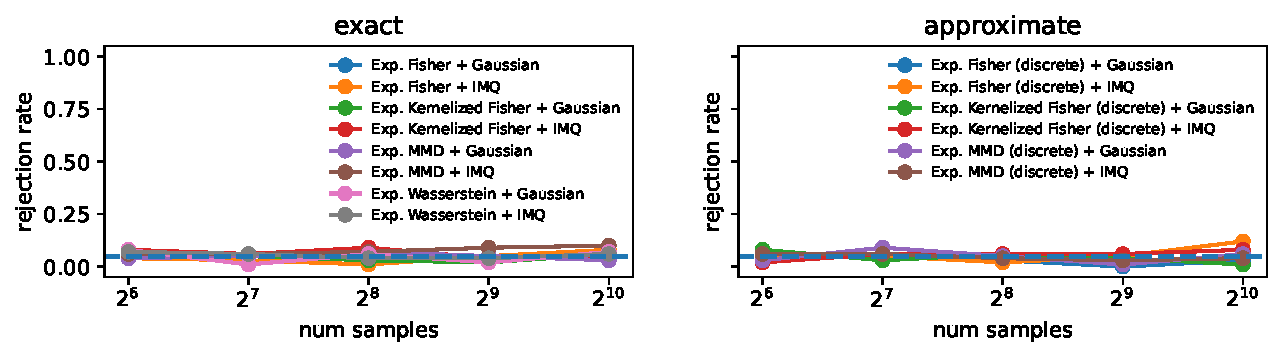
\includegraphics[width=\linewidth]{paper/figures/mgm_kccsd.pdf}
    \caption{False rejection rate of the KCCSD for MGM using exact and approximate (10 base samples) evaluations.}
    \label{fig:mgm_kccsd}
\end{figure*}

Figures~\ref{fig:mgm_kccsd} and \note{F.1} demonstrate that the proposed KCCSD tests are calibrated and their type I errors do not exceed the set significance level, apart from sampling noise.
We see that this holds both when we evaluate the kernels exactly, exploiting closed-form expressions for Gaussian distributions, and when we approximate the kernel evaluations using samples from the base measure.
The comparison with SKCE (\note{Figures~F.2 and F.3}) highlights that for the SKCE exact computations of the test statistic are only possible for specific combinations of models and kernels (in this example, Gaussian distributions with Gaussian kernels).

\subsection{Test Power}

We compare the test power of the proposed tests in different scenarios with the test power of SKCE-based tests.
We generate uncalibrated data with the following models:

\paragraph{Miscalibrated Mean Gaussian Model (MMGM)}
Here $\mathcal{X} = \mathcal{Y} = \mathbb{R}^d$, $\mathbb{P}(X) = \mathcal{N}(0, I_d)$, $\mathbb{P}(Y \,|\, X = x) = \mathcal{N}(x, I_d)$, and $P_{|x} = \mathcal{N}(x + \delta, I_d)$ for some $\delta \neq 0$.
We consider perturbations $\delta$ of the form $\delta_0 \bm{1}_d$ (miscalibration of all dimensions) and $\delta_0 e_1$ (miscalibration of only the first dimension) with different scales $\delta_0 > 0$.
A similar model was used by \citet{widmann2022calibration}.

\paragraph{Heteroscedastic Gaussian Model (HGM)}
Here $\mathcal{X} = \mathbb{R}^d$, $\mathcal{Y} = \mathbb{R}$, $\mathbb{P}(X) = \mathcal{N}(0, I_d)$, $\mathbb{P}(Y \,|\, X = x) = \mathcal{N}(\sum_{i=1}^d x_i, 1)$, and $P_{|x} = \mathcal{N}(\sum_{i=1}^d x_i, \sigma^2(x))$ where $\sigma^2(x) = 1 + 10 \exp{(- \|x - c\|^2_2 / (2 \times 0.8^2))}$ for $c = 2/3 \,\bm{1}_d$.
This model was used by \citet{jitkrittum2020testing}.

\paragraph{Quadratic Gaussian Model (QGM)}
Here $\mathcal{X} = \mathcal{Y} = \mathbb{R}$, $\mathbb{P}(X) = U(-2, 2)$, $\mathbb{P}(Y \,|\, X = x) = \mathcal{N}(0.1 x^2 + x + 1, 1)$, and $P_{|x} = \mathcal{N}(x + 1, 1)$.
This model was used by \citet{jitkrittum2020testing}.

\begin{figure*}
    \centering
    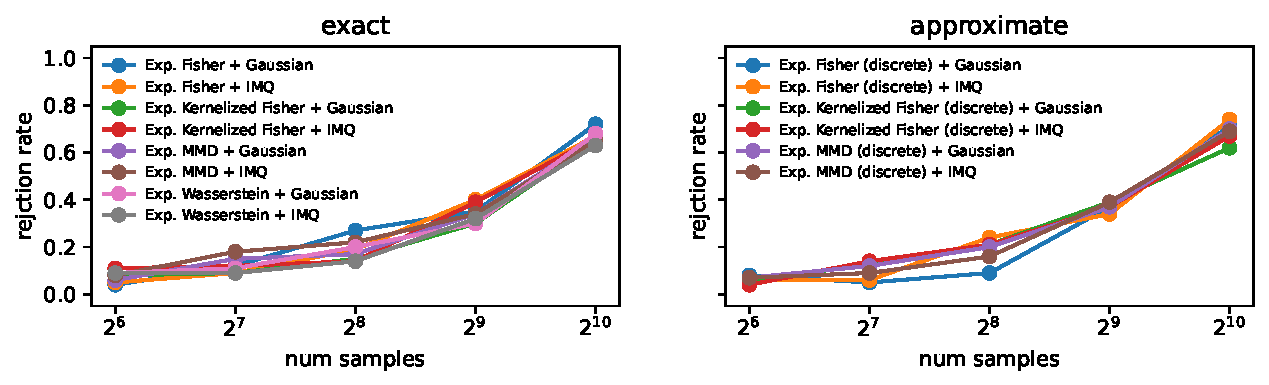
\includegraphics[width=\linewidth]{paper/figures/pmgm_kccsd_delta=0.1_shift-dim=1.pdf}
    \caption{Rejection rate of the KCCSD for MMGM ($\delta = 0.1 e_1$) using exact and approximate (10 base samples) evaluations.}
    \label{fig:mmgm_kccsd_first}
\end{figure*}

\section{Conclusion} \label{conclusion}


\begin{contributions} % will be removed in pdf for initial submission 
					  % (without ‘accepted’ option in \documentclass)
                      % so you can already fill it to test with the
                      % ‘accepted’ class option
    Briefly list author contributions. 
    This is a nice way of making clear who did what and to give proper credit.
    This section is optional.

    H.~Q.~Bovik conceived the idea and wrote the paper.
    Coauthor One created the code.
    Coauthor Two created the figures.
\end{contributions}

\begin{acknowledgements} % will be removed in pdf for initial submission,
						 % (without ‘accepted’ option in \documentclass)
                         % so you can already fill it to test with the
                         % ‘accepted’ class option
    Briefly acknowledge people and organizations here.

    \emph{All} acknowledgements go in this section.
\end{acknowledgements}

% References
\bibliography{refs}
\end{document}
